\section[Aktivační analýza]{Druhy a metody neutronové aktivační analýzy, pracovní procedury a praktické aplikace neutronové aktivační analýzy}

\textbf{Neutronová aktivační analýza} je radioanalytická metoda založená na jaderné aktivaci chemických prvků přítomných v analyzovaným vzorku. Patří mezi nejcitlivější chemické analýzi.

Existují i další aktivační analýzy založené na primárních fotonech, jiných nabitých částicích či vysokoenergetických neutronech, nicméně ty jsou komplikovanější (ale zase mohou objevit jiné prvky). NAA je totiž citlivá na velikosti účinných průřezů na daných prvcích (pokud je účinný průřez dostatečný, je možné zaznamenat i nepatrné stopové množství). Nejčastěji se tedy využívá neutronová analýza s tepelnými neutrony, kde jsou velmi vysoké účinné průřezy (n,$\gamma$) reakcí.

\begin{figure}[H]
    \centering
    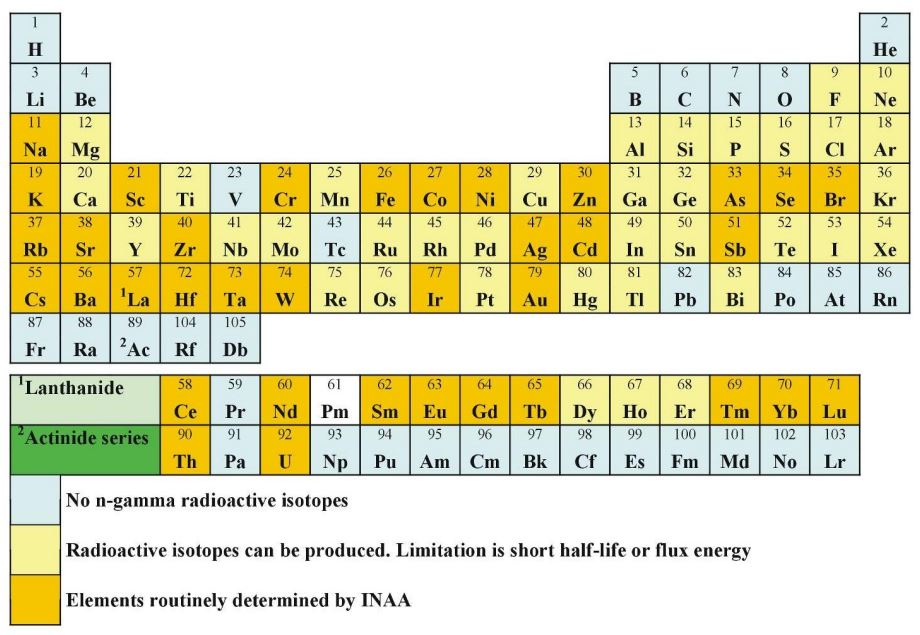
\includegraphics[width=0.65\textwidth]{img/prvky_NAA.JPG}
    \caption{Prvky vhodné pro NAA.}
\end{figure}

\subsection{Základní dělení}

Rozlišujeme:

\begin{itemize}
    \item \textbf{Kvalitativní NAA} -- zajímá mě pouze, které prvky se ve vzorku nacházejí.
    \item \textbf{Kvantitativní NAA} -- zajímá mě, v jakém množství se prvky ve vzoru nacházejí.
\end{itemize}

Dále dle energie neutronů (lze ovlivnit filtry): tepelné, epitermální, rychlé.

\subsubsection{Absolutní NAA}

Pokud známe přesnou hustotu neutronového toku a průběh účinného průřezu, tak je možné ze znalosti reakční rychlosti přesně dopočíst hmotnost zkoumaného izotopu. Hustotu toku ale přesně většinou neznám, proto se moc nevyužívá. Ale je vhodná, pokud dopředu nevím co hledám.

\begin{equation}
    \boxed{
        m = \dfrac{S \lambda \dfrac{t_\text{real}}{t_\text{live}}}{I_\gamma \: \varepsilon_\text{FEP}^\text{abs} \: \left( 1 - e^{-\lambda t_a} \right) e^{-\lambda t_v} \left( 1 - e^{-\lambda t_\text{real}} \right) \dfrac{N_A}{M} \int \sigma(E) \phi(E) \: \text{d}E}.
    }
\end{equation}

\subsubsection{Porovnávací NAA}

Pokud dopředu vím, co hledám, tak spolu se vzorkem ozářím etalon z daného materiálu o známé hmotnosti. Za předpokladu rovnosti produkčních rychlostí ve vzorku i v etalonu pak přes trojčlenku dopočtu množství izotopu ve vzorku. Vyhnu se neznalosti neutronového toku a účinných průřezů, ale pro každý izotop musím mít vlastní standard a oboje ozařovat za stejných podmínek.

\begin{equation}
    \boxed{
        m = m_\text{et} \dfrac{P}{P_\text{et}}.
    }
\end{equation}

\subsubsection{Metoda jednoho komparátoru}

Něco mezi přímou a porovnávací metodou. Využívá tzv. k-faktory pro jednotlié prvky, tedy poměr ozářených aktivit mezi standartem a daným prvkem. Tyto faktory se pak určují buď výpočtem (složité), nebo experimentálně (společným ozářením). Experimentálně získané k-faktory jsou pak přesnější, ale je možné je využít pouze pro daný detektor, reaktor a geometrii a za předpokladu stabilního neutronového pole. Jsou nepřenositelné.

Pak stačí spolu se vzorkem ozářit pouze etalon se standardem a za pomoci dopředu známých k-faktorů určit i-tý prvek.

\begin{equation}
    \boxed{
        m = k_i m_\text{com} \dfrac{P}{P_\text{com}}.
    }
\end{equation}

\subsubsection{Metoda $k_0$ standardizace}

Zdokonalení předchozí metody, k porovnávání jsou využity $k_0$ faktory, které jsou přenositelné. Spolu se vzorkem se ozáří komparátor (zlato), ke kterému jsou tabelovány hodnoty $k_0$ a $Q_0$.

\begin{equation}
    \boxed{
        m = m_\text{com} \dfrac{P \: I}{P_\text{com} \: I_\text{com}} \dfrac{1}{k_0} \dfrac{1 + \dfrac{Q_0^\text{com}}{f}}{1 + \dfrac{Q_0}{f}}, \: \: \: f = \dfrac{\phi_\text{th}}{\phi_\text{epi}}.
    }
\end{equation}

Hodnoty $\phi_\text{th}$ a $\phi_\text{epi}$ se pak stanoví aktivačním měřením neutronového pole za pomoci změření reakčních rychlostí v tepelné a epitermální oblasti na zlatém komparoátoru/standardu s a bez kadmiového filtru na základě \textbf{Hoghdalovy konvence}.

Platí, že spektrum v reaktoru je možné rozepsat do 3 složek (štěpné Wattovo, 1/v Fermiho a tepelné Maxwellovo), které je možné mezi sebou provázat pomocí empirických spojovacích funkcí. Konvence pak říká jak je možné stanovit reakční rychlosti v těchto grupách na základě měření s a bez kadmiového filtru (ještě třeba pronásobit kadmiovým faktorem, ten najdu na internetu):

$$ R_\text{th} = R - f_\text{Cd}R_\text{Cd}, $$
$$ R_\text{epi} = f_\text{Cd}R_\text{Cd}. $$

Potom platí:

$$ \phi_\text{th} = \dfrac{P_\text{th}}{g(T_0) \: \sigma_0 \: G_\text{th}}, $$
$$ \phi_\text{epi} = \dfrac{P_\text{epi}}{I_0 \: G_\text{epi}}, $$

kde $g(T_0)$ je opravný faktor pro oblast 1/v, $G$ je korekční faktor pro samostnínění, $sigma_0$ průřez pro (n,$\gamma$) reakci na etalonu při energii $E_0$ a $I_0$ je rezonanční integrál pro energii $E_0$:

\begin{equation}
    \boxed{
        m = m_\text{Au} \dfrac{P I}{P_\text{Au} I_\text{Au}} \dfrac{1}{k_0} \dfrac{G_\text{th,Au} f + G_\text{epi,Au} Q_{0\text{,Au}}}{G_\text{th} f + G_\text{epi} Q_{0}}, \: \: \: Q_0 = \dfrac{I_0}{\sigma_0}.
    }
\end{equation}

\subsection{Pracovní postup}

\begin{itemize}
    \item[1)] Vzorek připravím k ozáření (pevné vzorky přilepím izolepou, případně nějaká chemická separace biologických vzorků) a vložím do neutronového pole. Případně přidám etalon.
    \item[2)] Ozařuji vzorek po dobu $t_a$.
    \item[3)] Přenesu vzorek do laborky a připravím k měření (doba $t_v$).
    \item[4)] Změřím gamma spektrum (doba $t_\text{real}$) a určím produkční rychlosti jednotlivých FEP peaků.
    \item[5)] Dle konkrétní metody přepočtu produkční rychlost na hmotnost. Pokud má izotop vícero linek, tak provedu analýzu pro všechny peaky, ze kterých určím vážený průměr.
\end{itemize}

Měření je možné optimalizovat:

\begin{itemize}
    \item opakováním měření, 
    \item použití vícero peaků,
    \item delší doba měření $t_\text{real}$,
    \item kratší doba vymírání $t_v$,
    \item delkší doba aktivace $t_a$ (ideálně do saturovaného stavu),
    \item co nejmenší mrtvá doba,
    \item cyklicky ozařovat (nutné pro krátkodobě žijící izotopy, např. $^{20}$F. Pak je možné změřit i izotopy s poločasy rozpadu v jednotkách vteřin).
\end{itemize}


\subsection{Využití NAA}

NAA se uplatňuje v:

\begin{itemize}
    \item archeologie (kosti mamutů, nádobí),
    \item geologie (složení hornin, vyvřelin),
    \item historie,
    \item biomedicína,
    \item výživové produkty (složení doplňků stravy),
    \item průmysl,
    \item apod.
\end{itemize}

Jde o částečně destruktivní metodu (problém jsou živé organismy, které pravděpodobně umřou).